\section{Performance Evaluation}
\label{sec:simulation}
In this section, we will evaluate the performance of the proposed {\fwName} optimizer based on the data traces generated by the high-fidelity {\fwName} simulator. The road map of the {\fwName} simulator can be customized via CARLA \cite{CARLA}, and the typical \emph{Town01} map of CARLA is adopted as the simulation scenario. Moreover, the random traffic is generated via the \emph{activitygen} utility from SUMO \cite{SUMO}, where the parameters are configured as follows:
\begin{itemize}
    \item The total population is $1000$; $30\%$ in the age range $[0, 30]$, $50\%$ in the range $[30, 60]$, and $20\%$ in the range $[60, 90]$;
    \item The car holding rate is $58\%$, and the average time to drive $1$ kilometer is $360$ seconds;
    \item The working hour begins between 8:30AM and 9:00AM, and ends between 5:30PM and 6:00PM.
\end{itemize}
The simulator generates the 24-hour traffics across the whole map, and we choose the traffics from 8:30AM to 9:00AM to simulate the uplink model transmission.

In the uplink transmission, the length of one time slot is $2$ seconds and the maximum scheduling period is $200$ time slots, i.e., $T_s=2$ and $T_{\max}=200$ respectively.
There are $5$ {\IAVs}, each with a different pre-determined traffic route.
The number of remote antennas of the BS is $3$. The routes and locations of BSs are illustrated in Fig. \ref{fig:traffic_map}. The size of the model parameters is $750$ MBytes and the uploading bandwidth $B_0$ is $10$ MHz. The maximum transmission power of {\IAVs} is $P_{\max} = 5$ Watt. The typical channel parameters in urban area are adopted, i.e., the path-loss exponent $\epsilon=2.0$ and $\sigma=10.0$. Moreover,$T_{\text{comp},m}=0$ ($\forall m\in\carSet$) in the simulation.

\begin{figure}[htp!]
    \centering
    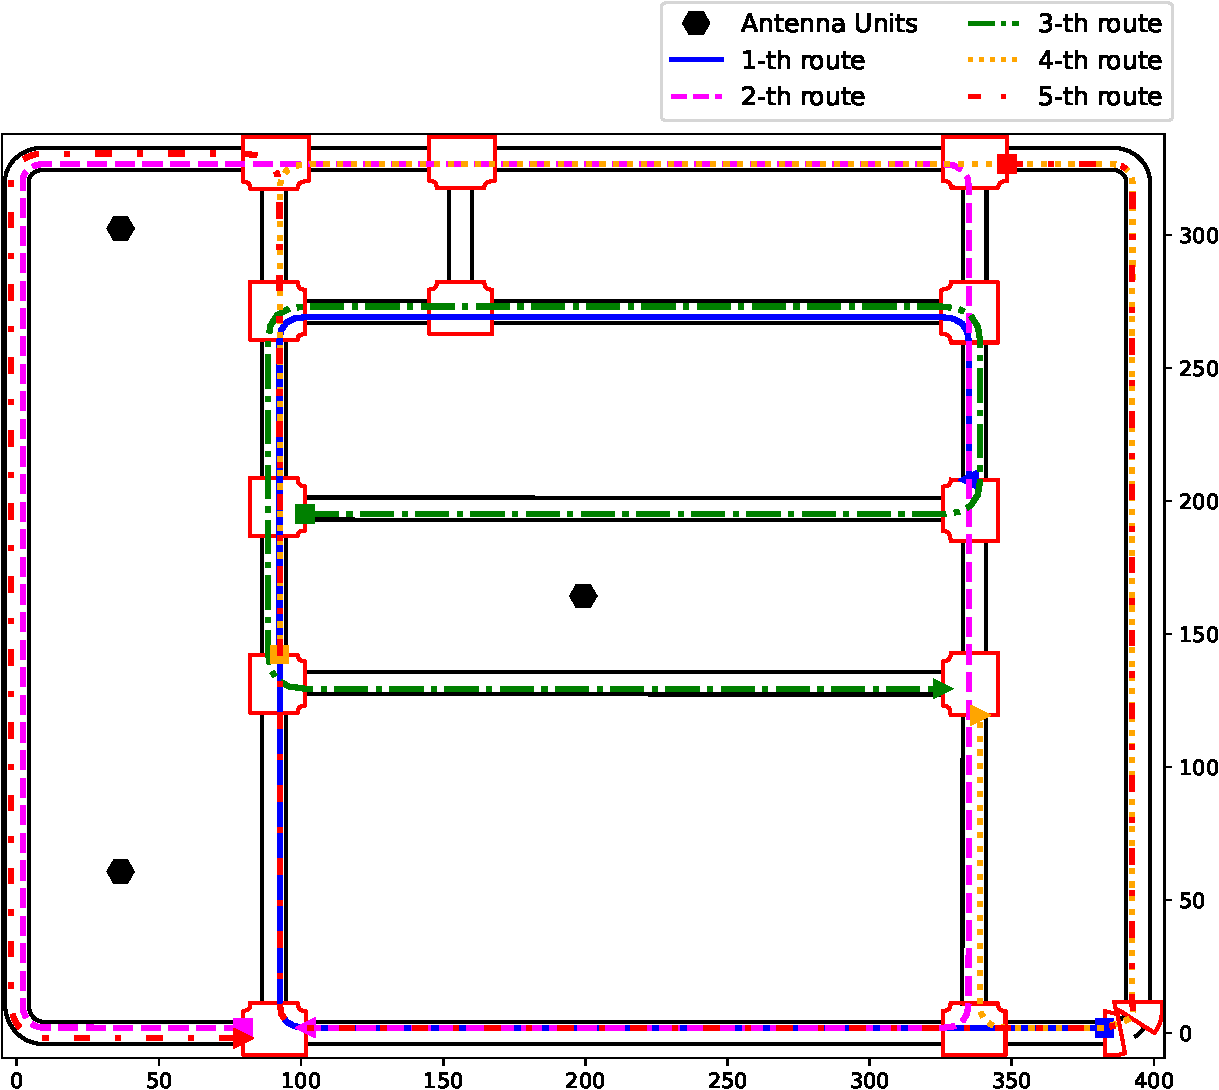
\includegraphics[width=0.45\textwidth]{fig_traffic_map.pdf}
    \caption{Illustration of the road map, {\IAV} routes, and BS locations.}
    \label{fig:traffic_map}
\end{figure}

In order to demonstrate the performance gain, we compare the proposed {\fwName} optimizer with the following benchmarks algorithms.
\begin{itemize}%<*tag:newpolicy>
    \item \revise{\textbf{Deterministic policy}: Solve the deterministic optimization problem \textbf{P2$(0)$} at the very beginning according to the average trajectories of {\IAVs}, and applied the solution in the scheduling of all the time slots.}%</tag:newpolicy>
    \item \textbf{Equal-time policy}: All the {\IAVs} are allocated with the maximum transmit power $P_{\max}$ and equal transmit time in each time slot.
    \item \textbf{Best-channel policy}: Always choose the {\IAV} with the best channel condition in each time slot, i.e., $\gamma_{m',t}=1$, $p_{m',t} = P_{\max}$, where $m' = \arg\min_{m} l_{m,t}$, $\forall t$.
    \item \textbf{Decoupled Policy}: Solve the deterministic optimization problem \textbf{P2$(0)$} at the very beginning according to the average trajectories of {\IAVs}, and apply local-slot scale optimization (problem \textbf{P3}) at each time slot based on the solution of \textbf{P2$(0)$}.
\end{itemize}

\subsection{Performance Analysis}
\label{subsec:performance}

The overall average performance of the proposed {\fwName} optimizer and the benchmarks is illustrated in Fig. \ref{fig:analyze_total_cost}, where each super slot consists of $5$ time slots.
All schemes are simulated with the same initial system state, and the average overall costs are compared. It can be observed that the average overall cost of the {\fwName} optimizer is significantly better than the equal-time policy and the best-channel policy.
\revise{
    The deterministic policy performs even worse than the equal-time policy. This is mainly because the distribution variance of {{\IAVs}}' future locations could be large at the very beginning of the scheduling. Hence, the scheduling optimization based on average trajectories may have a significant mismatch for the future time slots. Moreover, the decoupled policy performs much better than the deterministic policy.
    In the former, we use the time allocation of the deterministic policy, and apply local finite-horizon MDP to solve the power allocation for each {\IAV} respectively.
    The above performance gain demonstrates the significant benefit of dynamic programming, compared with the deterministic optimization, in the transmission with random trajectories.
}%
Finally, the performance gain of the proposed {\fwName} optimizer over the decoupled policy is due to periodic optimization of problem \textbf{P2}.


To further demonstrate the performance gap between the proposed {\fwName} optimizer and the benchmarks, we also plot the accumulated weighted cost versus time slots in Fig. \ref{fig:analyze_accumulated_cost}.


\begin{figure}
    \centering
    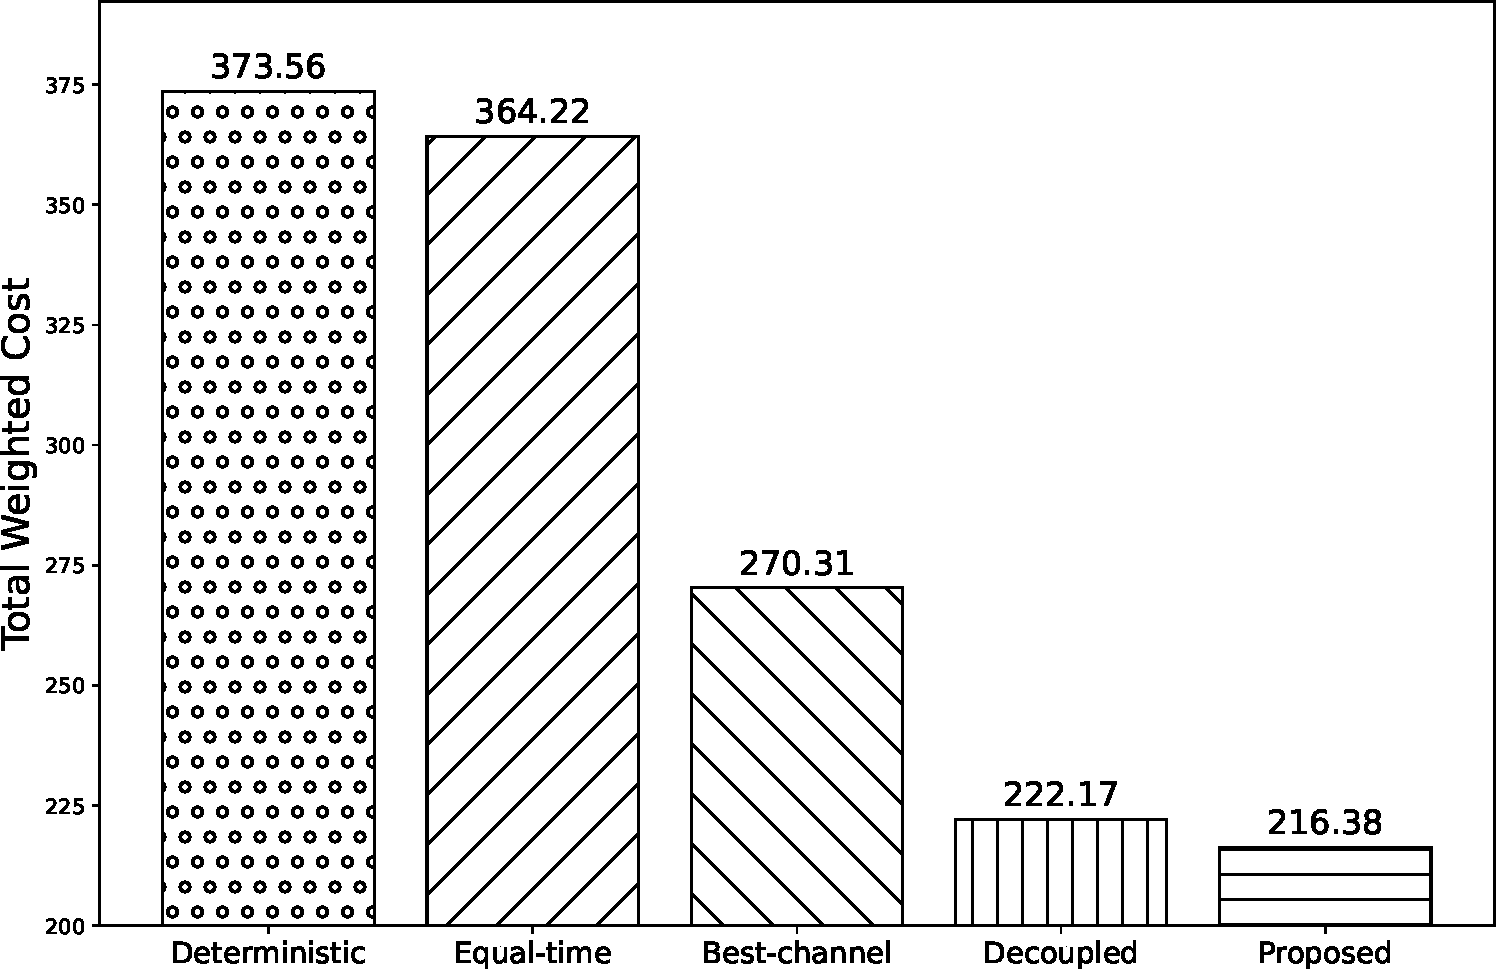
\includegraphics[width=0.45\textwidth]{analyze_cost_bar_new.pdf}
    \caption{\revise{The total weighted cost of the proposed {\fwName} optimizer and the benchmarks.}}
    \label{fig:analyze_total_cost}
\end{figure}

  
\begin{figure}
    \centering
    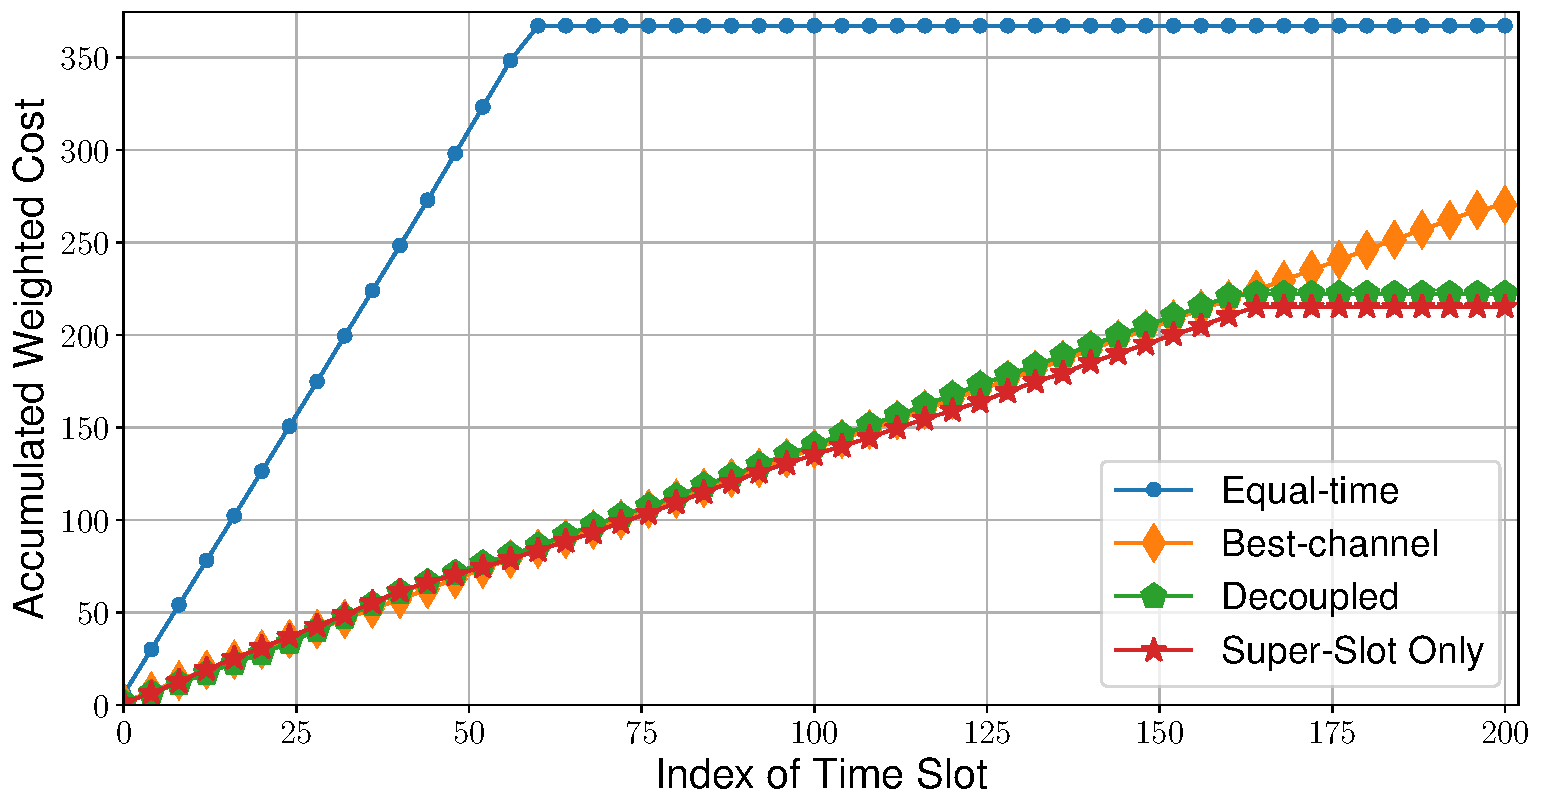
\includegraphics[width=0.45\textwidth]{analyze_accumulated_cost.pdf}
    \caption{The accumulated weighted cost versus time slots.}
    \label{fig:analyze_accumulated_cost}
\end{figure}


\subsection{Sensitivity Study}
\label{subsec:sensitivity}

In this part, the sensitivity of the performance of the proposed {\fwName} optimizer versus the system parameters is illustrated to demonstrate the robustness of the algorithm.

\noindent\textbf{Super Slot Length $N$:}
The average overall cost of the proposed {\fwName} optimizer versus different number of slots in one super slot is illustrated in Fig. \ref{fig:study_super_slot}. Smaller values of $N$ lead to more frequent super-slot scale optimization, and hence larger computational complexity. It can be observed that average overall cost decreases when decreasing $N$. Moreover, the cost suppression is trivial when $N\leq 10$.
\begin{figure}
    \centering
    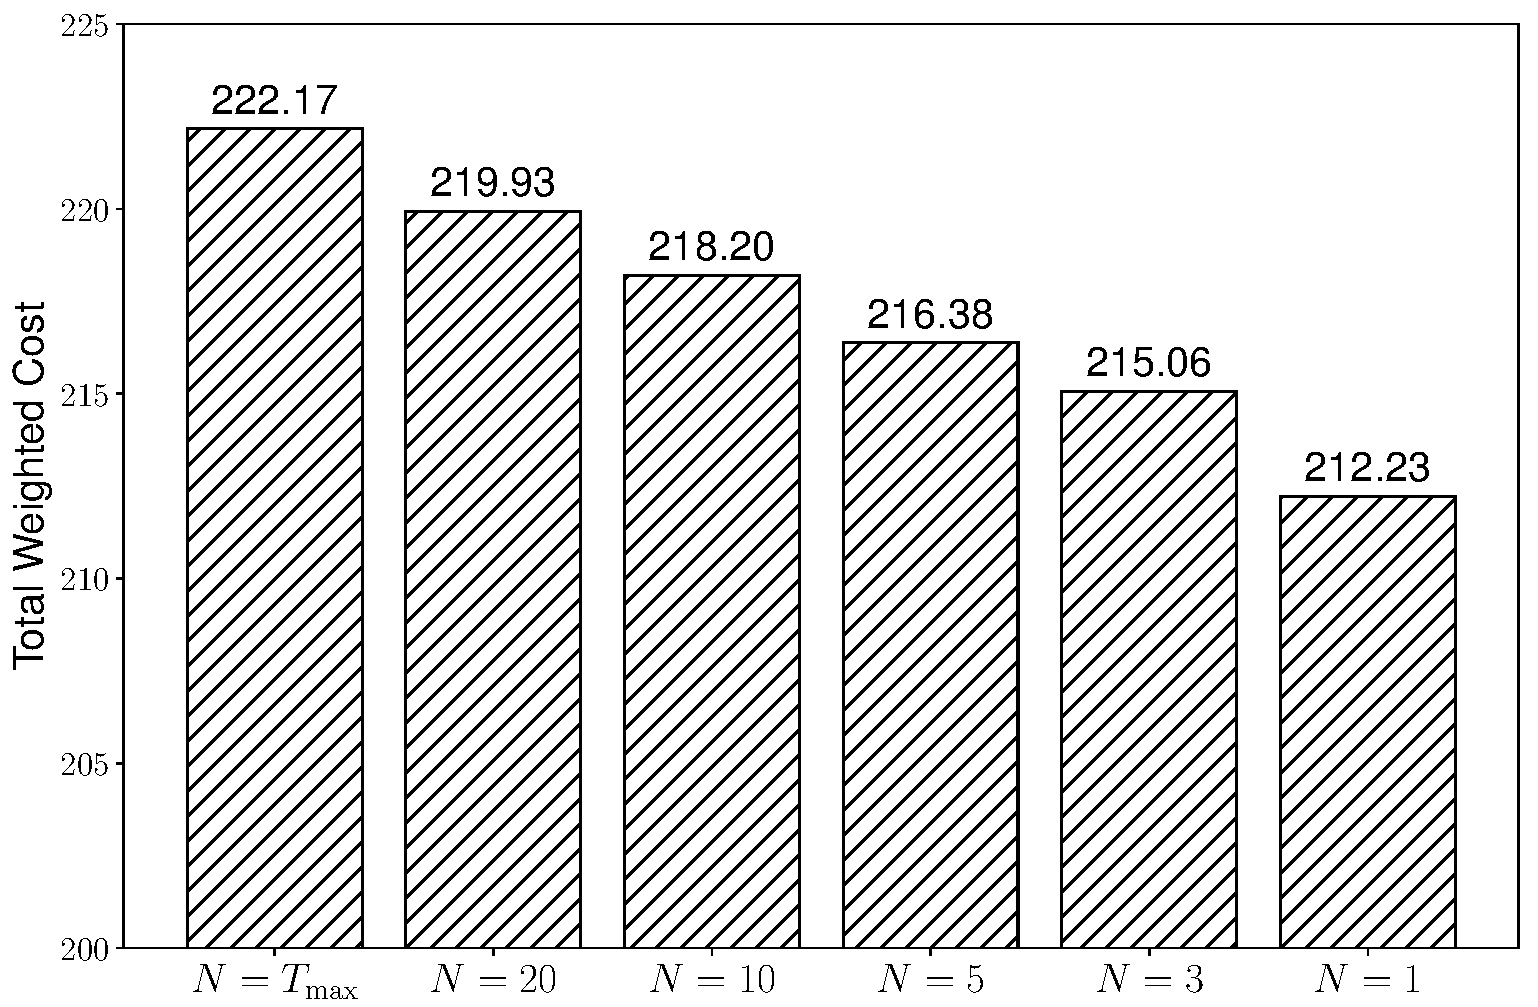
\includegraphics[width=0.45\textwidth]{study_super_slot.pdf}
    \caption{The total weighted cost w.r.t different super slot length $N$.}
    \label{fig:study_super_slot}
\end{figure}
The results show that smaller $N$ leads to better performance but higher computational complexity.

\noindent\textbf{Pareto Efficiency:}
In Fig. \ref{fig:study_pareto_efficiency}, the performance gain of the proposed {\fwName} optimizer versus different weight values $\omega$ is illustrated.
It can be observed that compared with the equal-time policy which only minimizes time consumption and the best-channel policy which only minimizes energy consumption, the proposed {\fwName} optimizer can always achieve a better trade-off between time and energy consumption.
\begin{figure}
    \centering
    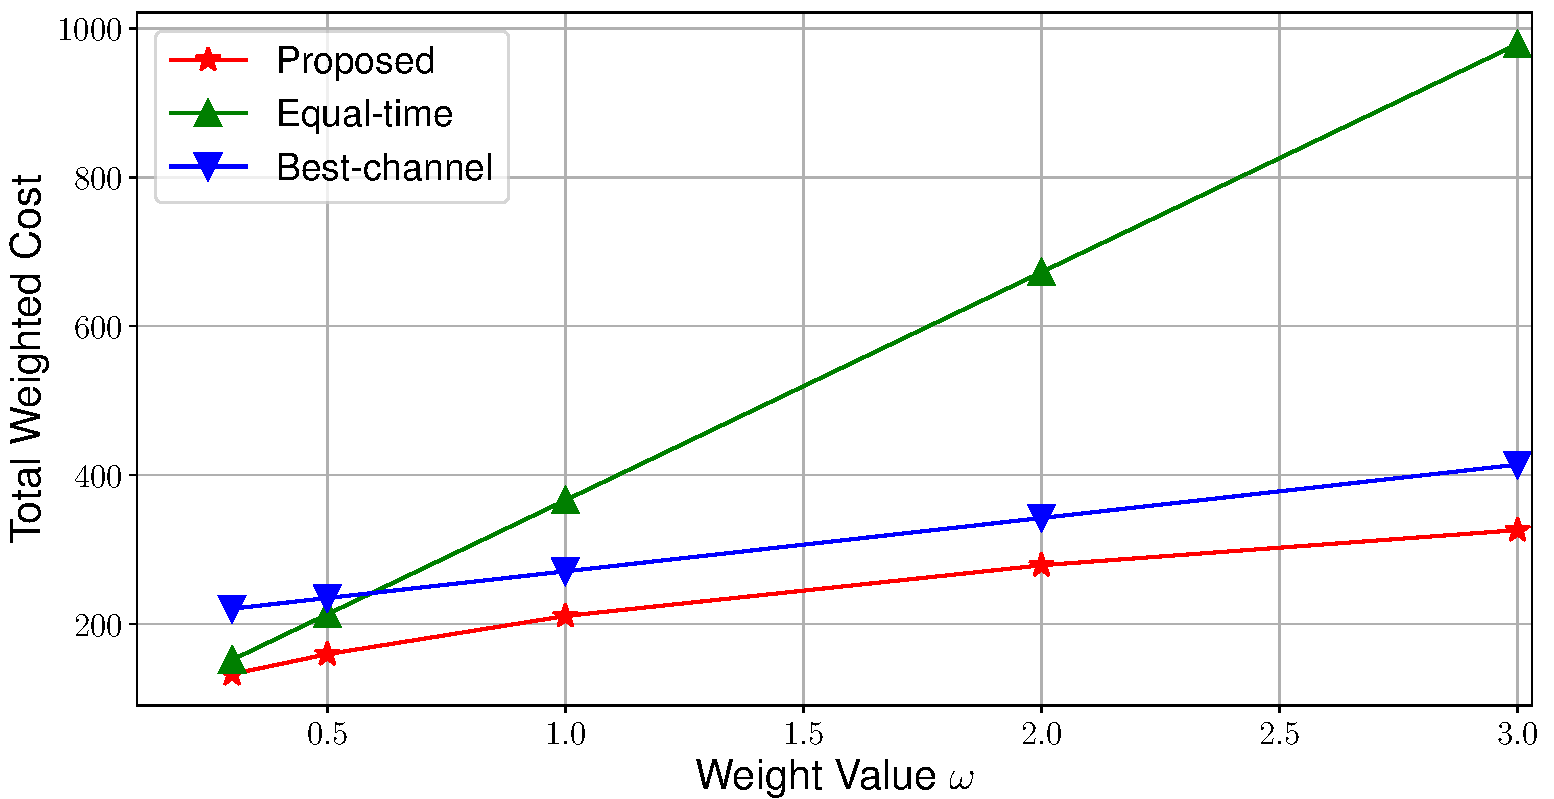
\includegraphics[width=0.45\textwidth]{study_pareto_efficiency.pdf}
    \caption{The total weighted cost of the proposed {\fwName} optimizer and the benchmarks under different weight values $\omega$.}
    \label{fig:study_pareto_efficiency}
\end{figure}
